\documentclass[intlimits,twoside,a4paper,11pt]{article}

% these settings specify the language and the file encoding

\usepackage[utf8]{inputenc}
\usepackage[T2A]{fontenc}

%Здесь дописана дополнительная опция english
%Add additional option: "english"
\usepackage[eqsecnum,authorsinfo,english]{kioj4}

% set first page
\setcounter{page}{42}

% journal sections, uncomment only first, if unknown
\journalsectionnoimage{}
%\journalsection{algorithmic-mathematics}
%\journalsection{informatics}
%\journalsection{mathematical-modeling}

% issue year, issue number, journal type: CAM = computer assisted mathematics journal
\issue{2015}{-}{cam}
\udknumber{621.320}

\title[Paper title]{PAPER TITLE}

\authorI[Andreev А.~\affil{1,2}]{Andreev Andrew}
\authorIpos{Ph.D.}
\authorIemail{aaa@org.com}
\authorIorcid{orcid.org/0000-0002-0261-3113}

\authorII[Borisov B.~\affil{2}]{Borisov Boris}
\authorIIpos{Ph.D.}
\authorIIemail{bbb@org.com}

\affiliation{1}{The first university, address, city, post index, country}
\affiliation{2}{The second university, address, city, post index, country}

\begin{document}

    \maketitle

    \begin{abstract}
        An abstract in English. Some abstract in English. An abstract in English. Some abstract in English. An abstract in English. Some abstract in English. An abstract in English. Some abstract in English. An abstract in English. Some abstract in English. An abstract in English. Some abstract in English. An abstract in English. Some abstract in English. An abstract in English. Some abstract in English. An abstract in English. Some abstract in English.
        \keywords keywords in English, more keywords in English
        \autocitationexample
        %\citationexample Andreev A.~A., Borisov B.~B. Template for the KIO journal, not published anywhere
        \acknowledgements here we may thank everybody who helped authors with this paper, and name grants that supported the research and the paper.
    \end{abstract}

    \section{INTRODUCTION}
    Some English text, some English text, Some English text, some English text, Some English text, some English text, Some English text, some English text, Some English text, some English text, with proper hyphenation. Very extermination extermination extermination extermination extermination extermination extermination extermination word, and anyway with the hyphenation.

    \section{FIRST SECTION}
    Some English text, some English text, Some English text, some English text, Some English text, some English text, Some English text, some English text, Some English text, some English text, with proper hyphenation.
    \begin{itemize}
        \item Itemization exmaple.
        \item The second point.
        \item The third point.
    \end{itemize}

    And now for something completely different:
    \begin{enumerate}
        \item The first point;
        \item The second point;
        \item The third point.
    \end{enumerate}
    Reference to the image~\ref{fig-example}

    \begin{figure}[htb]
        \centering
        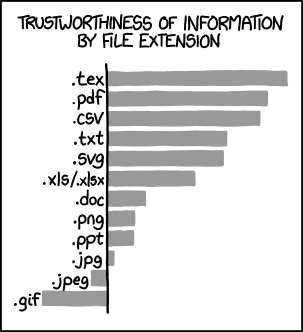
\includegraphics[width=0.4\textwidth]{xkcd1301.png}
        \caption{Trustworthness of information by file extension} \label{fig-example}
    \end{figure}

    \begin{table}[H]
        \centering
        \caption{Table example}
        \label{table-example}
        \begin{tabular}{|c|c|}
            \hline
            Question & ? \\
            \hline
            Answer & 42 \\
            \hline
        \end{tabular}
    \end{table}

    \subsection{A subsection}
    Text in subsection
    \subsubsection{A sub-subsection}
    Text in subsection with an example of an image consisting of two images. We can reference the full image, for example,~\ref{fig-example-2}, or subimages, for example,~\ref{fig-example-2b}.

    \begin{figure}[H]
        \centering
        \begin{subfigure}[t]{70mm} %указываем размер подрисунка, без буквы [t] картинки будут вертикально отцентрованы
            %we specified a subfigure width. Without the [t] option images will be vertically centered
            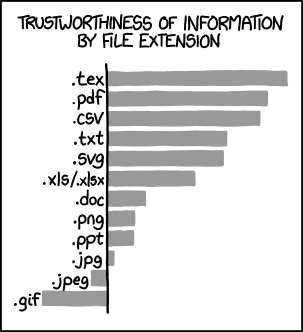
\includegraphics[width=\textwidth]{xkcd1301.png} %width=\textwidth указывает, что ширина совпадает с шириной подрисунка
            %width=\textwidth specifies, that width of the included image is equal to the subimage width.
            \subcaption{Unnecessary subcation}
            \label{fig-example-2a}
        \end{subfigure}
        \quad %это широкий пробел между двумя рисунками, this is a wide space between subfigures
        \begin{subfigure}[t]{50mm}
            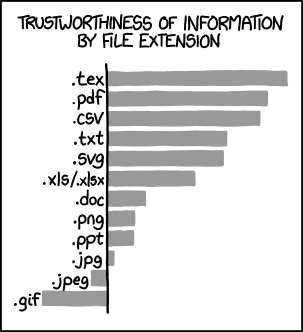
\includegraphics[width=\textwidth]{xkcd1301.png}
            \subcaption{} % Здесь подзаголовок не указан, no subcaption
            \label{fig-example-2b}
        \end{subfigure}
        \caption{An example of two images next to each other at the same figure} \label{fig-example-2}
    \end{figure}

    \section{CONCLUSION}
    Some conslusion text with a reference:~\cite{lib-1,lib-2}

    \begin{thebibliography}{9}
        \bibitem{lib-1} {\it Madhav S.} Game Programming Algorithms and Techniques: A Platform-Agnostic Approach (Game Design). UK, 2013.
        \bibitem{lib-2} {\it Ericson C.} Real-Time Collision Detection. USA, 2004.
    \end{thebibliography}

    \additionalinfo{additional info, some grant information, if needed}
    \additionalinfo{Received October 7, 2001, The final version: December 28, 2015}

    % no more text here

\end{document}
